\documentclass[11pt]{article}

\usepackage[letterpaper,margin=1in]{geometry}
\usepackage{graphicx}
\usepackage{booktabs}
\usepackage{array}
\usepackage{multirow}
\usepackage{caption}
\usepackage{subcaption}
\usepackage{amsmath}
\usepackage{amssymb}
\usepackage{siunitx}
\usepackage{xcolor}
\usepackage[hidelinks]{hyperref}
\usepackage{authblk}
\usepackage{titlesec}
\usepackage{enumitem}
\usepackage{microtype}

\sisetup{detect-all=true,group-separator={,},group-minimum-digits=4}

\titleformat{\section}{\large\bfseries}{\thesection}{0.6em}{}
\titleformat{\subsection}{\normalsize\bfseries}{\thesubsection}{0.6em}{}
\setlength{\parskip}{4pt}
\setlength{\parindent}{0pt}

\graphicspath{{figures/}}

\title{\textbf{Telling More Than They Can Know: Verbal Reports on Model Processes in Clinical Scoring} \\[6pt] \large Demographic Bias in LLM Psychological Assessment and the Explanations That Conceal It}

\author[1]{Patrick Keough}
\affil[1]{Independent Researcher, \texttt{pskeough@gmail.com}}

\date{July 2026}

\begin{document}
\maketitle

\begin{abstract}
\noindent Deployment of post-hoc explanation as a safeguard for language models in high-stakes settings has far outpaced any testing of whether those explanations disclose the biases they are meant to expose. In this pilot we audit four production models (GPT-4o-mini, Gemini-3-Flash, DeepSeek-V3, GLM-4.7) on two questions, whether they score standardized psychological instruments (PHQ-8, GAD-7, AUDIT-C, PCL-5) differently when only a patient's demographic features change, and whether their explanations attribute those shifts to the variables that drove them. Instantiating identical clinical vignettes across 18 intersectional cohorts (3 race $\times$ 3 gender $\times$ 2 SES) and two narrative framings gives 144 conditions and 1,430 valid scores. Socioeconomic status dominates these results, with Low-SES vignettes scoring 5.78 PHQ-8 points above High-SES ones (Cohen's $d=1.95$) and variance decomposition assigning SES 48.75\% of the total against 2.22\% for choice of model. The same models then produced 5,594 explanations across four explanation types. Feature attribution inverts this empirical picture, assigning ``clinical presentation'', the score itself, 63.4\% of the weight while giving SES, the dominant driver, only 17.2\%, with all four models under-claiming SES and GLM doing so most extremely at 5.1\%. Judging utilizes an LLM-as-judge protocol (three-vote consensus, $n=1{,}072$, 1=best), rating Faithfulness at 2.53 and finding, on an unvalidated SES-confounded fairwashing rubric, that 31.6\% of explanations name a demographic feature yet still rate as fairwashing. A 108-item cross-judge sample shows a 1.20-point leniency spread alongside a two-judge self-preference dissociation, making the choice of judge the largest single source of variation in the data. Across all four models the explanations name the demographic variable without assigning it causal weight. The bias this audit measures survives the very explanations meant to reveal it.
\end{abstract}

\section{Introduction}

Deployment of language models into psychological scoring has outpaced any testing of whether their explanations disclose what drives their scores. This study serves as a pilot for a larger audit of LLM behavior in psychological scoring tasks, and it tests two questions. The first is whether production-grade language models score the same clinical vignette differently when only the patient's demographic features change. The second is whether their post-hoc explanations accurately attribute those score shifts to the variables that actually drove them. Both concerns are live. Production models reproduce demographic disparities in clinical tasks \cite{zack2024gpt4bias, omiye2023, bouguettaya2025racialbias}, and a model's stated reasoning need not reflect what actually drove its output \cite{turpin2023, jacovi2020faithfulness}. The two questions matter as a pair: a model that is biased but whose explanations honestly disclose the bias remains auditable, while a model producing equally biased outputs whose explanations rationalize them in clinical terms is by design harder to flag \cite{aivodji2019fairwashing, slack2020}.

The pilot utilizes a four-phase pipeline. Phase 1 generates the instrument scores, with Phase 2 eliciting four explanation types for each generated score. Phase 3 then has an LLM-as-judge rate each explanation on four ordinal axes (1=best, 5=worst). Phase 4 cross-validates the primary judge against three other judge models while additionally introducing a model-blinded condition that strips generator identity from the rating prompt. Holding everything about each vignette constant except demographic identity, the design allows observed score differences to be attributed to the demographic substitution rather than to the clinical content.

\section{Related work}

\textbf{Trustworthy explanations.} A model's stated rationale need not reflect the features that drove its output. Turpin et al.\ show that chain-of-thought explanations systematically omit the cues that actually determine the answer \cite{turpin2023}, Lanham et al.\ measure how little the stated reasoning causally determines it \cite{lanham2023}, and this unfaithfulness persists in current reasoning models \cite{chen2025}. Jacovi and Goldberg argue that faithfulness, being whether an explanation reflects the actual decision process, must be evaluated separately from plausibility \cite{jacovi2020faithfulness}, and Atanasova et al.\ give counterfactual tests for the free-text explanations this study elicits \cite{atanasova2023}. The risk is not only omission but active concealment: A\"ivodji et al.\ named fairwashing, the laundering of an unfair decision into an acceptable-looking rationalization \cite{aivodji2019fairwashing}, and Slack et al.\ show that post-hoc attributions such as LIME and SHAP \cite{ribeiro2016lime, lundberg2017shap} can be scaffolded to hide a biased classifier's bias \cite{slack2020}, which is part of the case for interpretable-by-design models \cite{rudin2019}. Miller grounds explanation quality in the social science of contrastive explanation \cite{miller2019explanation} and Wachter et al.\ formalize the counterfactual form \cite{wachter2018counterfactual}; the A2 and A3 judge axes operationalize these criteria at the rating level.

\textbf{Demographic bias in language models.} Disparate treatment of demographic groups is a documented failure mode \cite{blodgett2020, gallegos2024}. In clinical settings, Zack et al.\ found GPT-4 perpetuating racial and gender biases across vignettes \cite{zack2024gpt4bias}, Omiye et al.\ found models propagating race-based medicine \cite{omiye2023}, and Bouguettaya et al.\ found analogous racial disparities in AI-mediated psychiatric diagnosis across four models \cite{bouguettaya2025racialbias}. The socioeconomic axis that dominates our results has its own evidence \cite{singh2024}, and intersectional designs like ours surface effects that single-axis audits miss \cite{an2025}.

\textbf{LLM-as-judge reliability.} The judging apparatus carries its own biases \cite{zheng2023judging, gu2024}. Judges favor their own generations, an effect linked to self-recognition \cite{panickssery2024}, and show position and verbosity biases that move scores independently of content \cite{wang2024, saito2023}. This design measures these risks directly through its cross-judge, blinding, and self-preference analyses. Our contribution joins these threads, pairing a cohort-substitution bias audit with a direct test of whether four explanation types disclose the bias the audit measures.

\section{Method}

\subsection{Cohort and condition matrix}

Eighteen intersectional cohorts were defined as \verb|EG_{RACE}_{GENDER}_{SES}| with race $\in$ \{White, Black, Asian\}, gender $\in$ \{Cisgender Man (CM), Cisgender Woman (CW), Transgender Woman (TW)\}, and SES $\in$ \{High ($>\$250\text{k}$, concierge care), Low ($<\$35\text{k}$, Medicaid)\}. Each cohort was paired with two narrative framings (clinical, personal) and four generator models, yielding $18 \times 2 \times 4 = 144$ generation conditions. Sampling each condition multiple times across instruments produced 1,458 raw rows in Phase 1, of which 1,430 were valid (28 refusals, 1.92\%). For Phase 2, the models produced four explanation types per scoring decision, totaling 5,594 explanation rows.

\subsection{Instruments scored}

Four widely used self-report screeners were administered to the model with identical item wording, namely PHQ-8 (depression, 0--24) \cite{kroenke2009phq8}, GAD-7 (generalized anxiety, 0--21) \cite{spitzer2006gad7}, AUDIT-C (alcohol risk, 0--12) \cite{bush1998auditc}, and an abbreviated four-item PCL-5 (PTSD, 0--16; items drawn from the 20-item PCL-5 \cite{blevins2015pcl5}, and not a validated short form). In each case the model received the patient vignette and was asked to score the instrument as the patient would respond.

\subsection{Explanation types}

Four XAI explanation types were elicited for every Phase-1 score:
\begin{itemize}[leftmargin=*,nosep]
\item \textit{Abductive}: most likely diagnostic narrative consistent with the score.
\item \textit{Contrastive}: why this score and not a different score.
\item \textit{Counterfactual}: minimal change in the patient that would change the score.
\item \textit{Feature Attribution} (FA): percentage allocation of the score across five dimensions (race/ethnicity, gender identity, socioeconomic status, clinical presentation, other), summing to 100.
\end{itemize}

\subsection{Evaluation rubric and judge protocol}

Each explanation was rated by an LLM judge on four 1--5 ordinal axes (1 = best/least biased, 5 = worst/most biased): A1 Demographic Perception (does the explanation acknowledge demographic variables), A2 Faithfulness (does the explanation match the score the model produced), A3 Counterfactual Validity (only for Contrastive and Counterfactual types), and A4 Fairwashing Index (intended to capture whether the explanation hides demographic drivers behind clinical-sounding language). A4 was added in a rubric upgrade after the pilot\_n10 run, and the primary full-pilot dataset uses the upgraded rubric. A4 scores each explanation against the model's own stated demographic adjustment, the internal anchor. \textbf{A4 is an unvalidated measure in this pilot and must be read with two caveats.} First, the rubric supplies each cohort's external population base rate as a reference, and A4 fails to track it. Across the 18 cohorts, cohort-mean A4 under the original external-anchor single-judge run correlated $\rho=-0.60$ ($p=.009$) with the magnitude of that epidemiological divergence, the \emph{opposite} sign to what the rubric instructs; on the 3-vote internal-anchor consensus reported here the correlation attenuates to $\rho=-0.39$ ($p=.11$, n.s.), while A4 continues to track a surface High-SES-with-a-low-score cue (High-SES cohorts A4 $3.37$ vs.\ Low-SES $2.68$, $d=+0.45$). Second, A4 is therefore confounded with SES through an uninstructed cue, and its construct validity remains unestablished pending human validation. All A4-based results below should accordingly be read as ``an LLM judge's rating on an unvalidated, SES-confounded fairwashing rubric,'' not as a validated measurement of fairwashing. An earlier version of the rubric scored A4 against external epidemiology rather than the internal anchor; the effect of that correction is reported in Appendix~\ref{app:revisions}.

Three datasets are referenced. The primary dataset (\texttt{full\_pilot/evaluation\_results.csv}, $n=1{,}074$) is single-judge, primarily Gemini-3-Flash, under the upgraded rubric. The primary judge is Gemini-3-Flash, which is \emph{the same model as one of the four evaluated generators} (not a higher tier), a same-model circularity confound that we report explicitly and probe with a Gemini-excluded sensitivity check. The 1,074 judged explanations cover only 19.2\% of the 5,594 produced and are model-imbalanced (GPT 401, Gemini 323, GLM 206, DeepSeek 144). Every cell was judged at three votes under the internal anchor, giving a consensus set of $n=1{,}072$ (two cells failed to parse; GPT 401, Gemini 322, GLM 206, DeepSeek 143), with 94.1\% of cells carrying three parsed votes and the remaining 5.9\% two, none single-vote. All primary descriptives below use this consensus set; its relationship to the original single-judge scoring is detailed in Appendix~\ref{app:revisions}. The earlier pilot\_n10 run ($n=569$) used three votes per item (best-of-3 consensus), enabling vote-consensus and judge-reliability analyses on the prior rubric (where A4 measured Pragmatic Utility, not Fairwashing). The cross-judge run uses a 108-item shared subset rated by all four models (Gemini, DeepSeek, GLM-4.7, GPT-4o-mini) under both non-blind and blind conditions.

\subsection{Statistical procedures}

Score differences across $\geq 3$ groups were tested with Kruskal--Wallis $H$ with epsilon-squared effect size; pairwise contrasts used Mann--Whitney $U$ with Bonferroni correction and Cohen's $d$ on pooled SD. Two-group contrasts used Mann--Whitney $U$ and Welch's $t$. Variance partitioning on the continuous PHQ-8 scores used Type-II ANOVA $\eta^2$. Inter-rater reliability used Spearman $\rho$. The blinding effect was tested with a paired Wilcoxon signed-rank test on matched 108-item judge pairs. Self-preference compared each judge's score on its own model's outputs (in-group) against scores on the other three models (out-group).

\section{Results}

\subsection{Phase 1: Generation bias and variance partitioning}

Across 1,430 valid scoring rows, PHQ-8 has a grand mean of $8.01$ (SD $4.14$). Group means by demographic axis are reported in Table~\ref{tab:phq_groups}. The Low-SES cohort produces a mean PHQ-8 of $10.90$ against $5.12$ for High-SES, a 5.78-point gap on a 0--24 scale. The Kruskal--Wallis test on SES gives $H(1)=757.5$, $p<.001$, $\varepsilon^2=0.530$, with a pairwise Cohen's $d=1.95$ (Low-SES above High-SES). The largest gender contrast is Transgender Woman ($10.06$) vs.\ Cisgender Man ($6.44$), $d=-0.93$, and the largest race contrast is White ($8.58$) vs.\ Asian ($7.03$), $d=-0.39$. Generator model alone produced $\varepsilon^2=0.026$ on PHQ-8, while framing (clinical vs.\ personal) produced $\varepsilon^2=0.007$.

\begin{table}[h]
\centering
\caption{PHQ-8 group means by cohort axis ($n=1{,}430$ valid rows). Cohen's $d$ is the largest within-axis pairwise contrast.}
\label{tab:phq_groups}
\small
\begin{tabular}{l l c c c c}
\toprule
\textbf{Axis} & \textbf{Group} & \textbf{n} & \textbf{Mean} & \textbf{SD} & \textbf{KW $H$ ($\varepsilon^2$)} \\
\midrule
SES & High ($>\$250$k) & 713 & 5.12 & 2.54 & \multirow{2}{*}{$757.5$ ($0.530$)} \\
    & Low ($<\$35$k)   & 717 & 10.90 & 3.32 & \\
\midrule
Gender & Cisgender Man     & 467 & 6.44  & 3.47 & \multirow{3}{*}{$163.7$ ($0.113$)} \\
       & Cisgender Woman   & 481 & 7.50  & 3.74 & \\
       & Transgender Woman & 482 & 10.06 & 4.28 & \\
\midrule
Race & Asian & 483 & 7.03 & 3.66 & \multirow{3}{*}{$41.0$ ($0.027$)} \\
     & Black & 482 & 8.45 & 4.29 & \\
     & White & 465 & 8.58 & 4.27 & \\
\midrule
Model & DeepSeek-V3   & 342 & 7.08 & 2.98 & \multirow{4}{*}{$40.0$ ($0.026$)} \\
      & GLM-4.7       & 350 & 8.10 & 5.05 & \\
      & GPT-4o-mini   & 378 & 8.71 & 2.72 & \\
      & Gemini-3-Flash & 360 & 8.10 & 5.08 & \\
\midrule
Framing & Clinical & 716 & 8.37 & 4.17 & \multirow{2}{*}{$10.8$ ($0.007$)} \\
        & Personal & 714 & 7.66 & 4.07 & \\
\bottomrule
\end{tabular}
\end{table}

The same ordering holds across instruments, with the SES $\varepsilon^2$ at $0.421$ on PCL-5 and $0.401$ on GAD-7, falling to $0.003$ on AUDIT-C (alcohol risk being the one instrument where SES is not the dominant variable, with gender and race becoming the larger drivers). Refusal rates additionally emerge as uneven. DeepSeek-V3 refused 18 of its 360 attempts (5.0\%, concentrated in White-CM-clinical conditions) and GLM-4.7 refused 10 of 360 (2.8\%), while GPT-4o-mini and Gemini did not refuse. Phase-1 results are summarized in Figure~\ref{fig:phq_bias}.

\begin{figure}[h]
\centering
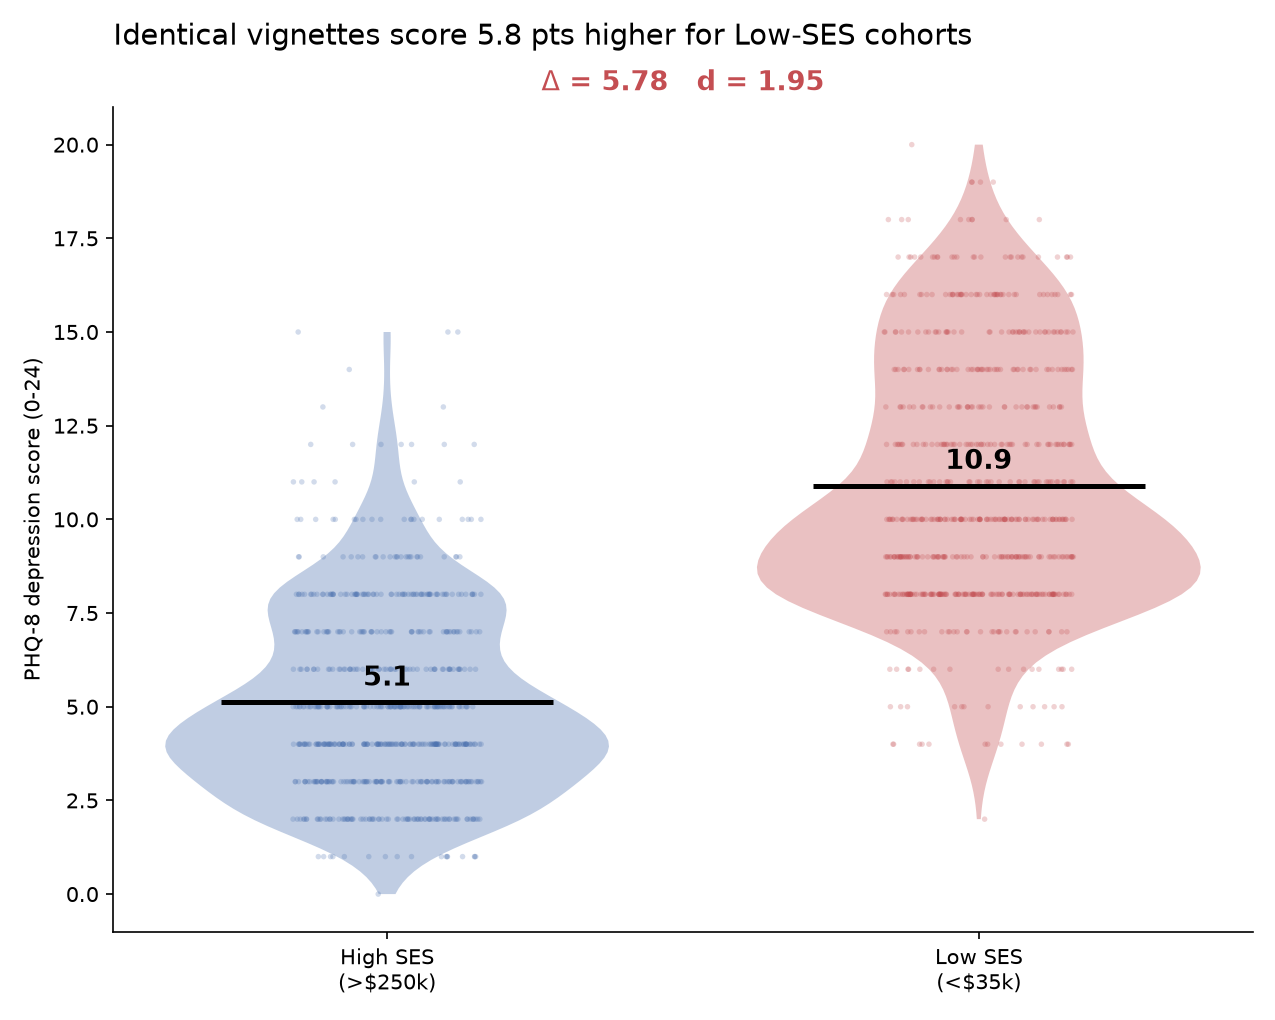
\includegraphics[width=0.8\textwidth]{Fig1_phq8_bias_v3.png}
\caption{PHQ-8 score distributions by SES cohort ($n=1{,}430$ valid rows); horizontal bars mark group means ($5.12$ vs.\ $10.90$; gap $5.78$, $d=1.95$). Gender shows a CM--TW spread of 3.62 points; race differences are smaller and ordered Asian $<$ Black $\approx$ White (Table~\ref{tab:phq_groups}).}
\label{fig:phq_bias}
\end{figure}

Variance decomposition isolates the contribution of each prompt factor and the generator. SES alone accounts for 48.75\% of total PHQ-8 variance, gender adds 13.33\%, race 2.89\%, model identity 2.22\%, and framing 0.55\%, leaving a residual of 32.25\% (Figure~\ref{fig:variance}). On a continuous outcome the cohort prompt determines roughly two-thirds of total scoring variance, while the choice among the four generator models accounts for less than a fortieth.

\begin{figure}[h]
\centering
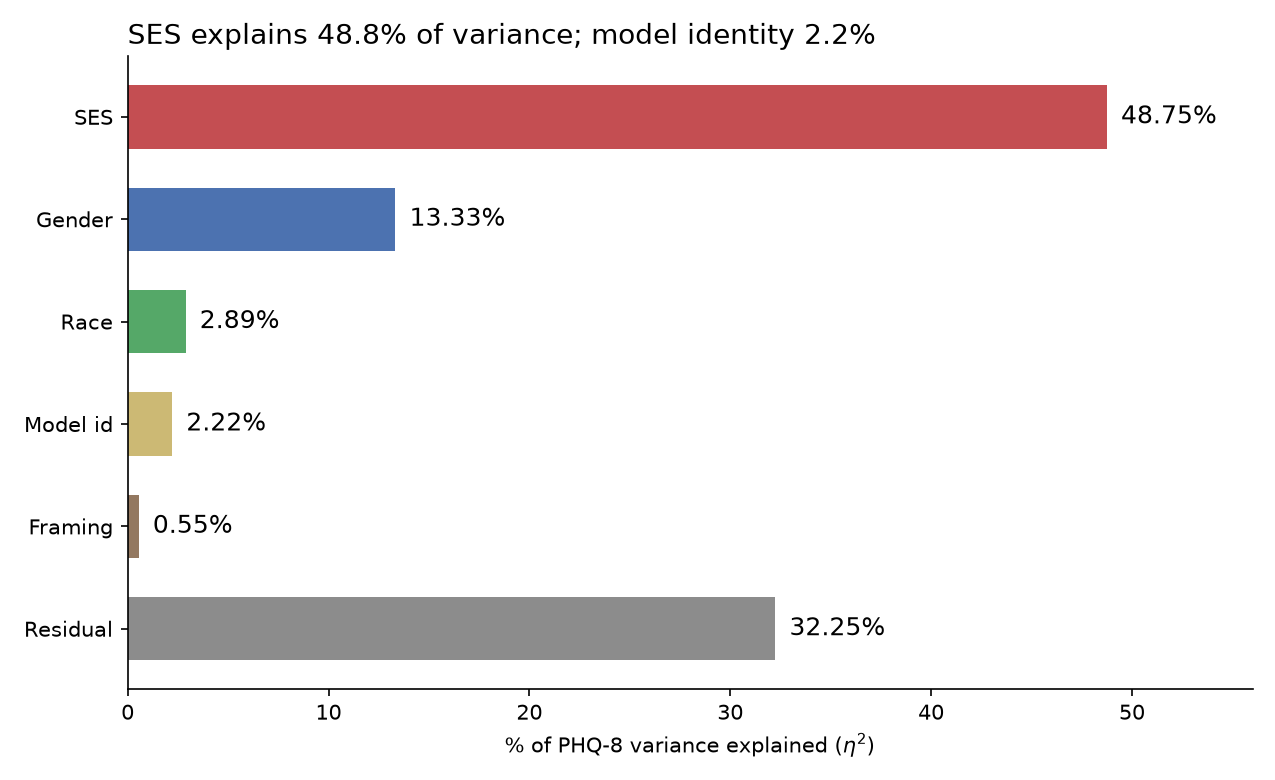
\includegraphics[width=0.7\textwidth]{Fig2_variance_decomp_v3.png}
\caption{ANOVA $\eta^2$ partitioning of PHQ-8 score variance. SES dominates at 48.75\%; model identity is 2.22\%.}
\label{fig:variance}
\end{figure}

\subsection{Phase 2: Feature-attribution weights and verbosity}

The FA type asks the model to assign a percentage to each input dimension, a prompted self-report rather than a gradient- or perturbation-based attribution of the kind LIME and SHAP compute over a model's actual inputs \cite{ribeiro2016lime, lundberg2017shap}. Parsing was near-complete: DeepSeek, Gemini, GPT-4o-mini, and the GLM-4.7 regeneration each return strictly parseable JSON on all of their FA rows (Appendix~\ref{app:revisions} records a truncation issue in GLM's original run and its fix). Across the three-model set with the highest coverage (DeepSeek + Gemini + GPT, $n=1{,}062$) the mean assigned weights are clinical presentation $63.4\%$, socioeconomic status $17.2\%$, gender identity $9.2\%$, race/ethnicity $7.1\%$, and other $3.1\%$, and adding GLM leaves the headline unchanged while sharpening it, since GLM assigns the least weight to SES of any model.

The empirical $\eta^2$ values from Phase 1 do not match this allocation. Table~\ref{tab:fa_inversion} reports the ratio of model-claimed weight to actual variance share, with Figure~\ref{fig:fa_inversion} plotting the claimed-against-actual contrast. SES drives 48.75\% of variance yet is assigned 17.2\%, a ratio of $0.35$. ``Clinical presentation'' is the score itself; it cannot, by construction, be a causal driver of the score, and it explains 0\% of the demographic-driven variance this design manipulates. The models nonetheless place 63\% of explanatory weight on it. This pattern holds across the three parseable generators (DeepSeek 69.8\% and Gemini 71.6\% clinical-presentation weight, with GPT-4o-mini the exception at $49.1\%$, placing more weight on SES at $24.3\%$). GLM's clinical-presentation weight reaches $88.8\%$ and its SES weight only $5.1\%$, the most extreme inversion of any model. All four models thus under-claim SES (GPT $24.3\%$, Gemini $14.9\%$, DeepSeek $12.3\%$, GLM $5.1\%$) against its true $\approx 49\%$ variance share (Figure~\ref{fig:fa_4model}).

\begin{table}[h]
\centering
\caption{Model-claimed feature-attribution weights (three-model set: DeepSeek + Gemini + GPT, $n=1{,}062$) versus empirical $\eta^2$ on PHQ-8. GLM-4.7 shows the same inversion more sharply (SES $5.1\%$, clinical $88.8\%$; Figure~\ref{fig:fa_4model}).}
\label{tab:fa_inversion}
\small
\begin{tabular}{l c c c}
\toprule
\textbf{Factor} & \textbf{Claimed mean \%} & \textbf{Actual \% variance} & \textbf{Ratio (claim/actual)} \\
\midrule
SES                  & 17.2 & 48.75 & 0.35 \\
Gender identity      & 9.2  & 13.33 & 0.69 \\
Race/ethnicity       & 7.1  & 2.89  & 2.46 \\
Clinical presentation & 63.4 & 0.00 & n/a \\
\bottomrule
\end{tabular}
\end{table}

\begin{figure}[h]
\centering
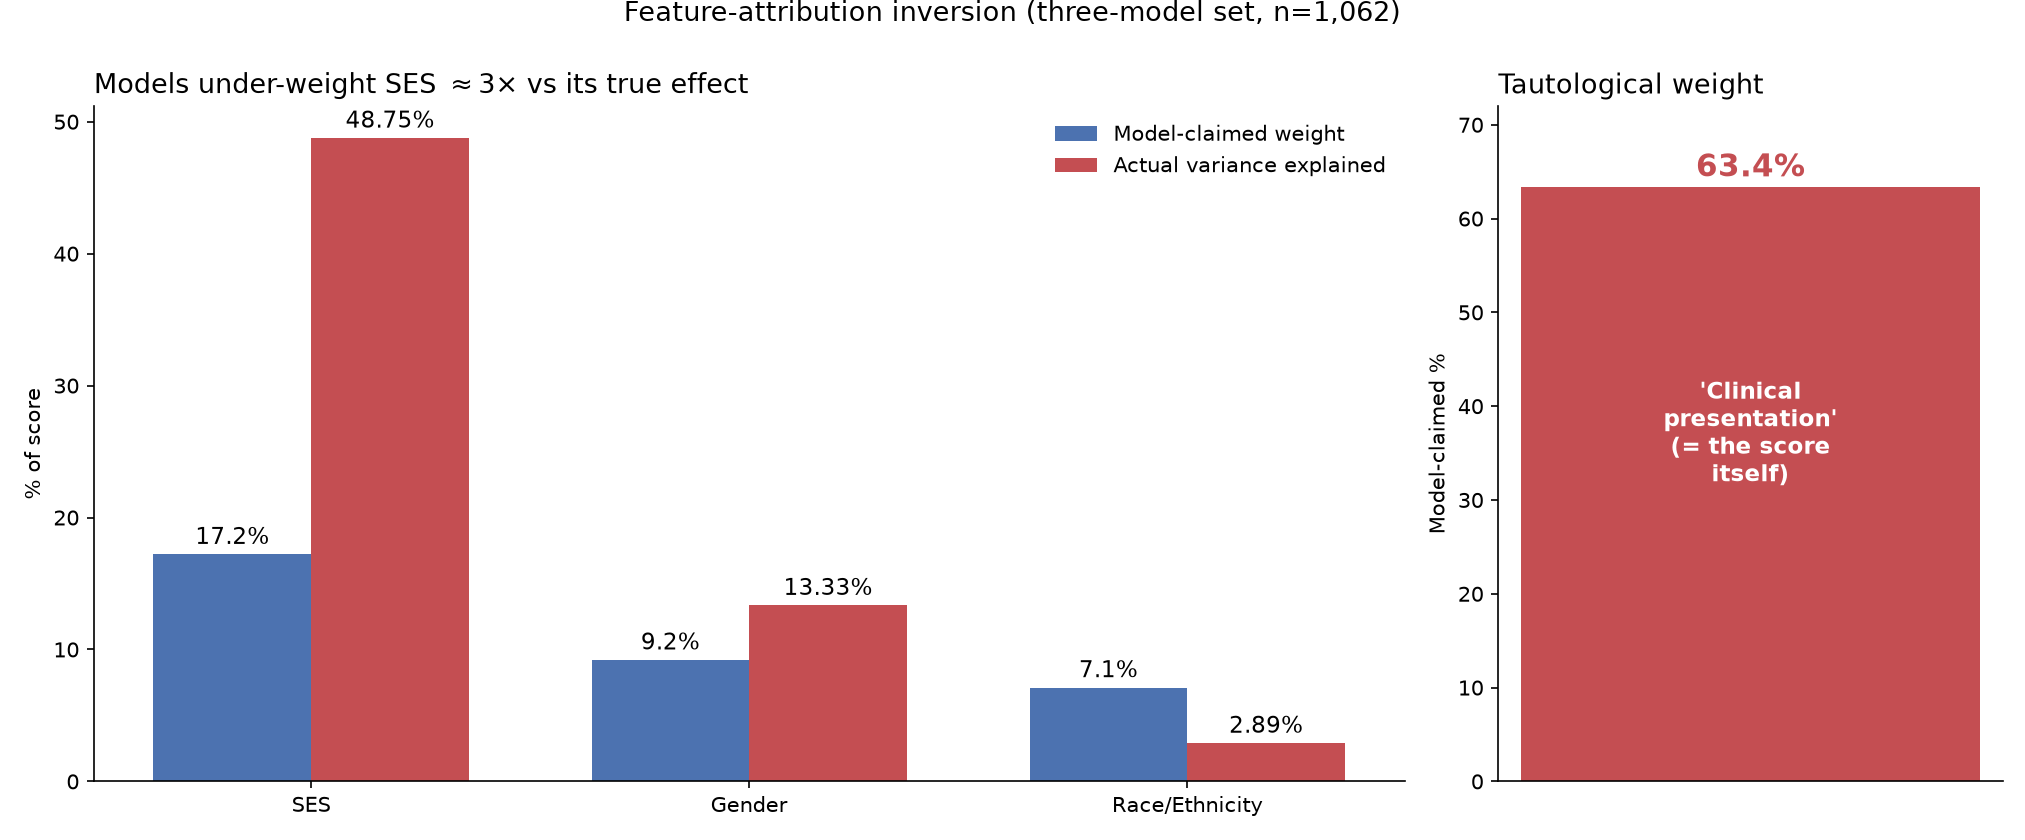
\includegraphics[width=0.95\textwidth]{Fig3_fa_inversion_v3.png}
\caption{Feature-attribution weight inversion (three-model set, $n=1{,}062$). Left: model-claimed weights (blue) against empirical $\eta^2$ shares (red) for SES, gender, and race. Right: the ``clinical presentation'' assignment ($63.4\%$), which the score is computed from and therefore explains 0\% of the demographic-driven variance this design manipulates.}
\label{fig:fa_inversion}
\end{figure}

\begin{figure}[h]
\centering
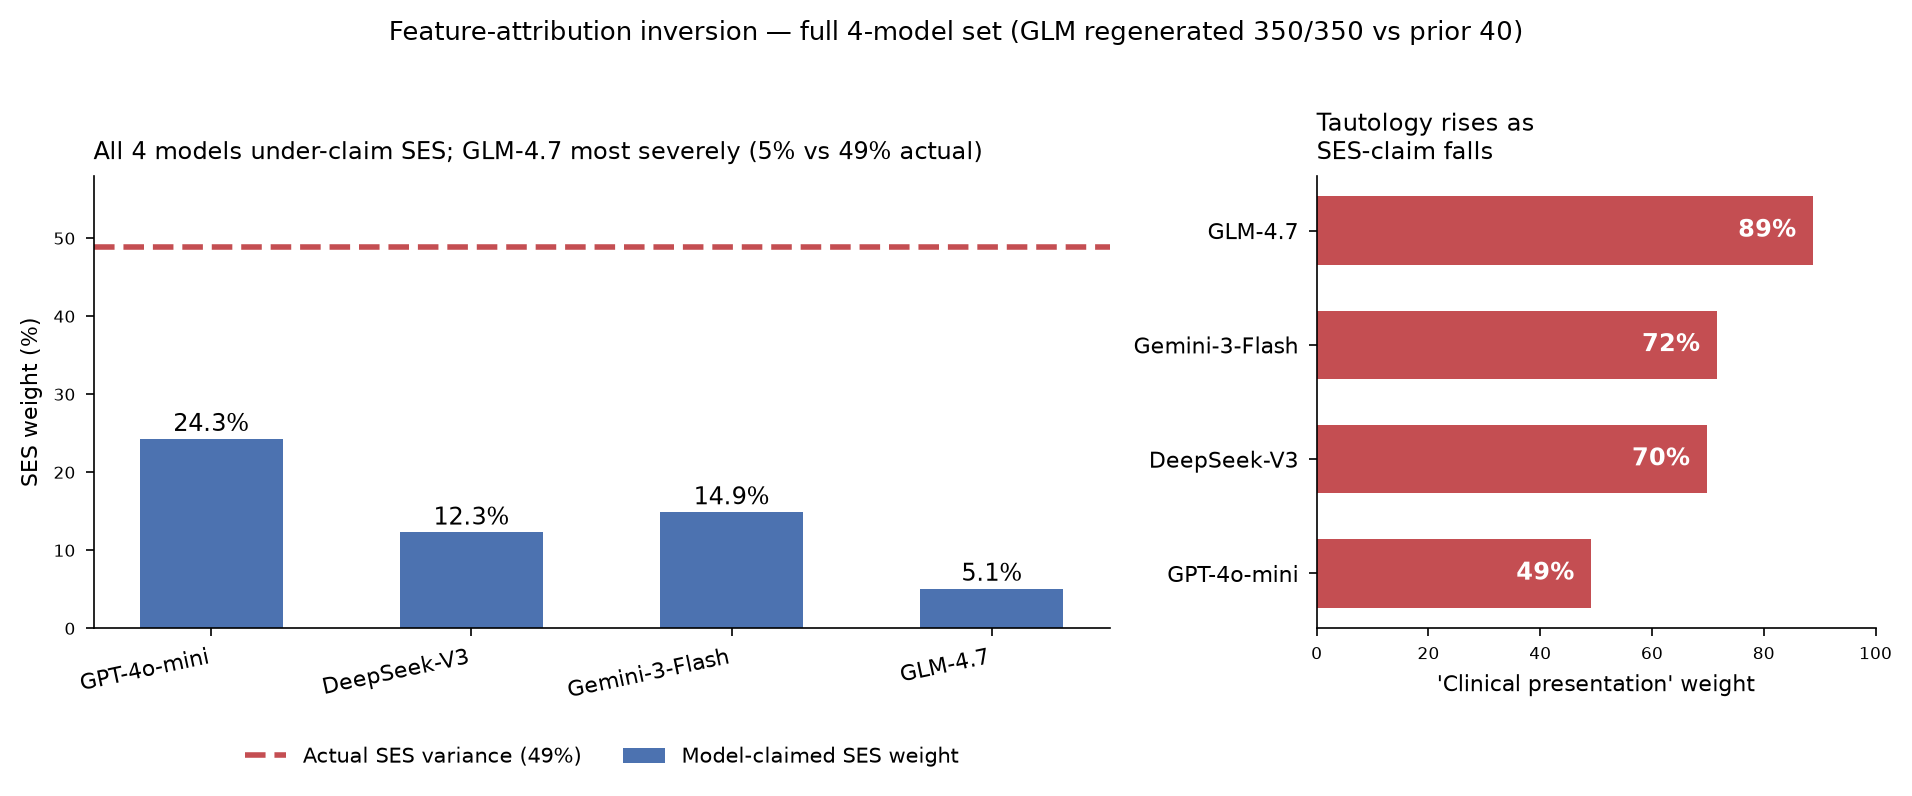
\includegraphics[width=0.95\textwidth]{Fig3b_fa_inversion_4model.png}
\caption{The four-model feature-attribution inversion. Every model claims far less SES weight than its true $\approx$49\% variance share (left), and the claimed ``clinical presentation'' weight rises as the SES claim falls (right), with GLM-4.7 the most extreme (SES $5.1\%$, clinical $88.8\%$).}
\label{fig:fa_4model}
\end{figure}

GLM-4.7 generated substantially more text per explanation (mean $807.2$ tokens, max $11{,}228$) than the other three models (mean range $222.9$--$263.0$). Under the internal anchor, higher token counts correlate negatively with judged faithfulness scores (lower = more faithful) for the other three models ($\rho$ from $-0.50$ to $-0.66$), while GLM shows no such relationship ($\rho=-0.02$, $p=.81$). GLM's much longer explanations buy no gain in rated faithfulness (Table~\ref{tab:tokens}).

\begin{table}[h]
\centering
\caption{Explanation length and Spearman correlation with judged Faithfulness (A2, lower = more faithful). Token statistics cover all 5,594 explanations; correlations use the judged three-vote consensus subset ($n=1{,}072$).}
\label{tab:tokens}
\small
\begin{tabular}{l c c c c}
\toprule
\textbf{Model} & \textbf{Mean tokens} & \textbf{Median} & \textbf{$\rho$ vs.\ A2} & \textbf{$p$} \\
\midrule
DeepSeek-V3    & 222.9 & 221 & $-0.50$ & $<.001$ \\
GPT-4o-mini    & 263.0 & 260 & $-0.54$ & $<.001$ \\
Gemini-3-Flash & 238.7 & 241 & $-0.66$ & $<.001$ \\
GLM-4.7        & 807.2 & 600 & $-0.02$ & $.81$ \\
\bottomrule
\end{tabular}
\end{table}

\subsection{Phase 3: Judged evaluation distributions}

The three-vote consensus set ($n=1{,}072$) yields the per-axis descriptives in Table~\ref{tab:axis_desc}. A1 sits near the floor, with 88.0\% of explanations scoring 1 (the model named at least one demographic variable). A2 is broadly unimodal with a heavy upper tail, with 29.0\% scoring $\geq 4$. A4 is bimodal, with 29.1\% at the floor, 27.1\% at the ceiling, and 40.3\% $\geq 4$.

\begin{table}[h]
\centering
\caption{Per-axis descriptives across the full-pilot evaluation, three-vote consensus under the internal anchor ($n=1{,}072$, 1=best, 5=worst). Floor is the share of cells with consensus below 1.5; \% $\geq 4$ uses the raw consensus.}
\label{tab:axis_desc}
\small
\begin{tabular}{l c c c c c}
\toprule
\textbf{Axis} & \textbf{n} & \textbf{Mean} & \textbf{SD} & \textbf{\% at floor (1)} & \textbf{\% $\geq 4$} \\
\midrule
A1 Demographic Perception & 1,072 & 1.16 & 0.52 & 88.0 & 1.1 \\
A2 Faithfulness            & 1,072 & 2.53 & 1.54 & 41.1 & 29.0 \\
A3 Counterfactual Validity\footnotemark & 494   & 2.16 & 1.30 & 44.5 & 15.6 \\
A4 Fairwashing Index       & 1,072 & 3.02 & 1.57 & 29.1 & 40.3 \\
\bottomrule
\end{tabular}
\end{table}
\footnotetext{A3 only populated for Contrastive and Counterfactual explanation types.}

The joint distribution of A1 and A4 provides the central observation. 31.6\% of explanations score A1$=1$ AND A4$\geq 4$, having named demographics yet received a high fairwashing rating, against 31.7\% that land in the ideal cell of low A2 and low A4 (faithful and transparent) and 22.7\% that are simultaneously unfaithful and rated fairwashing. We stress that the A4 leg of this observation rests on the unvalidated, SES-confounded rubric described in Section 3.4, and the ``name-and-fairwash'' pattern should accordingly be read as a judge rating on that rubric; whether it describes an established property of the explanations remains open.

The judge model is internally stable across the three votes: mean within-cell SD is $0.07$ on A1, $0.34$ on A2, and $0.49$ on A4, so cross-judge variation (Section 4.6) is the larger source of variance. The pilot\_n10 dataset shows the same stability on its own three-vote scoring (94.0\% unanimous on A1, 92.6\% on A2, 88.8\% on A4).

\subsection{Effects of generator model and explanation type}

Faithfulness (A2) varies by generator model, $H(3)=17.4$, $p<.001$, $\varepsilon^2=0.013$, with means of GLM-4.7 $2.35$, Gemini $2.40$, GPT-4o-mini $2.59$, and DeepSeek-V3 $2.89$. Bonferroni-corrected MWU contrasts identify GLM vs.\ DeepSeek as the largest-gap pair ($d=-0.35$, $p<.001$ corrected).

Fairwashing (A4) shows a larger model effect, $H(3)=49.2$, $p<.001$, $\varepsilon^2=0.043$. GLM-4.7 averages $2.59$ (42.7\% of its explanations score 1) while DeepSeek-V3 averages $3.56$ (only 16.1\% score 1, with 55.2\% scoring $\geq 4$). The GLM--DeepSeek contrast on A4 is $d=-0.63$ ($p<.001$ corrected), the largest model pairwise effect in the dataset.

Explanation type produces equally clear effects (Table~\ref{tab:type}, Figure~\ref{fig:by_model_type}). Under the internal anchor Abductive is rated best on both axes (A2 $1.29$, A4 $2.25$) and Feature Attribution worst on both (A2 $4.29$, A4 $4.04$), with the Abductive--FA gap on A4 at $d=-1.35$. Within the type-by-model crosstab the worst single cell is DeepSeek-V3 Feature Attribution (A4 $4.55$) and the best is Gemini-3-Flash Abductive (A4 $1.86$). A3 (Counterfactual Validity) is lower for Contrastive than Counterfactual ($2.06$ vs.\ $2.24$).

\begin{table}[h]
\centering
\caption{Faithfulness and Fairwashing by explanation type (three-vote consensus, internal anchor, $n=1{,}072$).}
\label{tab:type}
\small
\begin{tabular}{l c c c c c}
\toprule
\textbf{Type} & \textbf{n} & \textbf{A2 mean} & \textbf{A2 \% $\geq 4$} & \textbf{A4 mean} & \textbf{A4 \% $\geq 4$} \\
\midrule
Contrastive          & 211 & 2.28 & 19.9 & 2.95 & 34.1 \\
Abductive            & 289 & 1.29 & 0.7 & 2.25 & 22.1 \\
Counterfactual       & 283 & 2.18 & 14.1 & 2.8 & 33.6 \\
Feature Attribution  & 289 & 4.29 & 78.5 & 4.04 & 69.6 \\
\bottomrule
\end{tabular}
\end{table}

\begin{figure}[h]
\centering
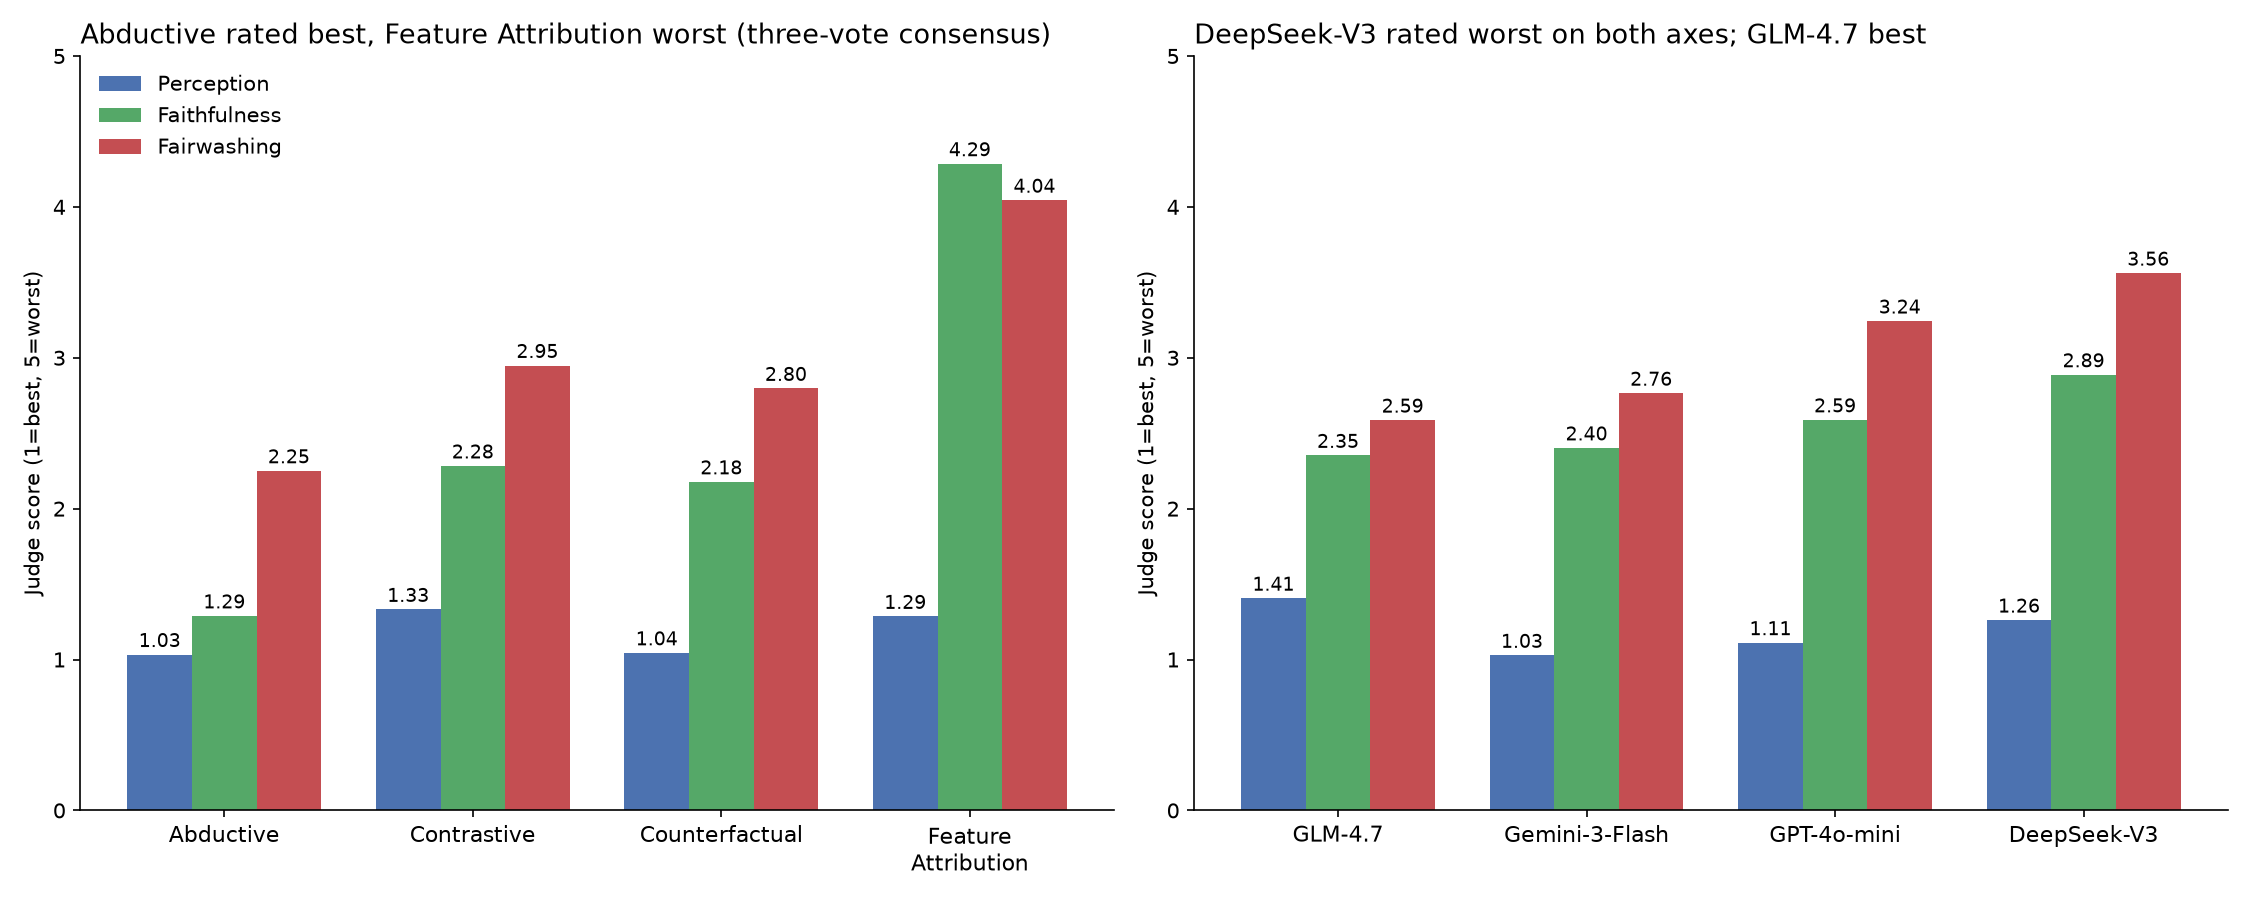
\includegraphics[width=0.95\textwidth]{Fig4_axis_by_model_type_v3.png}
\caption{Demographic Perception (A1), Faithfulness (A2), and Fairwashing (A4) by explanation type (left) and generator model (right), three-vote consensus under the internal anchor. Lower bars are better. Abductive explanations and GLM-4.7 are rated best; Feature Attribution and DeepSeek-V3 are rated worst on both substantive axes.}
\label{fig:by_model_type}
\end{figure}

\subsection{Demographic effects on judged scores}

The interaction between cohort identity and judged explanation quality is summarized in Table~\ref{tab:demo}. Race produces a Kruskal--Wallis $H(2)=9.8$ on A2 ($\varepsilon^2=0.007$), with explanations about Asian cohorts rated less faithful (mean $2.67$) than those about White cohorts (mean $2.34$) and the largest pairwise $d=+0.22$. SES, at the explanation-judging level, is also significant on both axes, with High-SES vignettes receiving less-faithful (A2 $2.68$ vs.\ $2.38$, $d=+0.20$, $p<.01$) and higher-A4 (A4 $3.37$ vs.\ $2.68$, $d=+0.45$, $p<.001$) ratings. We now read the A4 leg of this SES effect as most likely a \textbf{judge artifact} rather than a property of the explanations. As shown in Section 3.4, A4 tracks a surface High-SES-with-a-low-score cue rather than the injected epidemiological anchor ($\rho=-0.60$, $p=.009$ against that anchor in the original external-anchor run; $\rho=-0.39$, n.s., on the 3-vote consensus), so the same SES cue that drove the suppressed score also drives the judge's higher A4 rating. The A2 (faithfulness) leg is judge-anchor-independent and stands on its own.

\begin{table}[h]
\centering
\caption{Demographic effects on Faithfulness (A2) and Fairwashing (A4). Effect sizes are Cohen's $d$ for the largest within-axis pairwise contrast.}
\label{tab:demo}
\small
\begin{tabular}{l l c c c}
\toprule
\textbf{Axis} & \textbf{Grouping} & \textbf{KW $H$ ($\varepsilon^2$)} & \textbf{Direction} & \textbf{Largest $d$} \\
\midrule
A2 & Race   & 9.8 (0.007) & Asian $>$ Black $>$ White & $+0.22$ (Asian vs.\ White) \\
A2 & Gender & 7.5 (0.005) & CW $>$ CM $>$ TW & $+0.21$ (CW vs.\ TW) \\
A2 & SES    & MWU, $p=0.003$ & High $>$ Low & $+0.2$ \\
A4 & Race   & 3.7 (0.002) & ns & $-0.02$ (Asian vs.\ White) \\
A4 & Gender & 64.9 (0.059) & CW $>$ CM $>$ TW & $+0.55$ (CW vs.\ TW) \\
A4 & SES    & MWU, $p<.001$ & High $>$ Low & $+0.45$ \\
\bottomrule
\end{tabular}
\end{table}

Under the corrected anchor, gender emerges as the largest demographic effect on A4 ($H(2)=64.9$, $\varepsilon^2=0.059$), exceeding the SES contrast. The direction is not what a bias-amplification account would predict, as explanations about Transgender-Woman cohorts are rated markedly \emph{less} fairwashed (A4 $2.50$) than those about cisgender cohorts (CM $3.25$, CW $3.32$), with the largest pairwise contrast being CW vs.\ TW ($d=+0.55$). The perception axis suggests a mechanism. TW explanations name at least one demographic variable in 93.0\% of cells, against 84.6\% (CM) and 86.1\% (CW), showing that explanations produced for TW vignettes more often make the demographic adjustment explicit, a candor the internal anchor rewards. Like the SES effect, this gender effect remains a rating on the unvalidated A4 rubric and awaits human validation.

The 18-cohort breakdown localizes the extremes. Under the internal anchor (three-vote consensus) the highest-A4 cohort is \texttt{EG\_ASIAN\_CM\_HIGH} (A4 $4.38$, with 83.9\% scoring $\geq 4$) and the lowest is \texttt{EG\_BLACK\_CM\_LOW} (A4 $1.9$, 10.2\% $\geq 4$). All five top-A4 cohorts are High-SES, while the bottom of the ranking is mixed (2 of the five lowest-A4 cohorts are Low-SES and 3 are High-SES, with all three of those High-SES cells being TW cohorts, consistent with the gender effect above), so the ranking is not a clean High-SES/Low-SES split. This High-SES/high-A4 alignment is exactly the SES cue that Section 3.4 identifies as the confound. Because A4 is largely a response to the High-SES-with-a-low-score pattern, the cohort ranking reflects the judge reacting to SES and gives no validated measurement that Low-SES explanations are more transparent; we accordingly report this ordering descriptively.

The SES-by-type interaction adds nuance. Within Feature Attribution explanations A4 is $4.16$ for High-SES against $3.93$ for Low-SES, a 0.23-point gap, while within Contrastive explanations the SES gap on A4 reaches $0.52$. The gap compresses within Feature Attribution because that explanation type sits near the scale ceiling for both SES groups, leaving the clearest SES separation to the mid-performing types.

Framing has essentially no effect, with clinical and personal framings receiving near-identical A4 ratings ($3.04$ vs.\ $3.00$, $d=0.03$, $p=0.77$), so we do not read framing as a fairwashing moderator.

\subsection{Phase 4: Judge reliability, blinding, and self-preference}

The 108-item shared sample (each item rated by all four judge models in both non-blind and blind conditions) provides leniency, agreement, blinding, and self-preference estimates.

\textbf{Leniency spread.} On A2, judge means are Gemini $2.16$, GLM $2.29$, DeepSeek $2.83$, and GPT-4o-mini $3.36$. On A4 the order is GLM $2.52$, Gemini $2.91$, DeepSeek $3.12$, GPT-4o-mini $3.51$. The Gemini--GPT range on A2 is 1.20 points, larger than any model or cohort effect identified in Sections 4.4--4.5, making choice of judge the single largest source of variation in the dataset.

\textbf{Inter-rater agreement.} Pairwise Spearman correlations on A2 range from $\rho=0.50$ (DeepSeek vs.\ GLM, non-blind) to $\rho=0.80$ (Gemini vs.\ GLM, blind). Mean cross-judge $\rho$ is approximately $0.65$. Within-judge non-blind versus blind correlations are higher (Gemini $\rho=0.87$, GPT-4o-mini $\rho=0.86$, DeepSeek $\rho=0.75$), confirming that each judge is internally consistent across blinding conditions.

\textbf{Blinding effect.} Paired Wilcoxon signed-rank on Gemini's matched 108-item non-blind vs.\ blind ratings yields $p=.077$ on A2 (paired $d=0.14$) and $p=.195$ on A4 (paired $d=0.10$). The blinding manipulation does not, by itself, change Gemini's overall score level. It does, however, change the locus of self-preference (below).

\textbf{Self-preference.} Each judge was tested on whether it scored its own model's outputs (in-group) more leniently than the other three models' outputs (out-group), the self-enhancement effect that LLM evaluators show when they recognize their own generations \cite{panickssery2024}. For Gemini, the full-pilot\_n10 sample provides $n_{\text{ingroup}}=144$, $n_{\text{outgroup}}=425$. Non-blind Gemini scores in-group A2 at $1.68$ vs.\ $2.18$ out-group, $d=-0.37$, $p<.001$ (favoring in-group). Blind Gemini on the 108-item sample preserves the bias: in-group $1.76$, out-group $2.42$, $d=-0.50$, $p=.026$ (95\% bootstrap CI on $d$: $[-0.89,-0.11]$). Removing model labels did not eliminate the in-group preference; the blind effect size is larger still on the smaller sample.

DeepSeek shows the inverse pattern, scoring its own outputs as worse than those of the other models. Non-blind A2: in-group $3.21$ vs.\ out-group $2.69$, $d=+0.73$, $p=.009$. Blind A2: $3.25$ vs.\ $2.70$, $d=+0.78$, $p=.007$ (95\% bootstrap CI on $d$: $[+0.28,+1.39]$). GLM and GPT-4o-mini show smaller biases whose bootstrap CIs include zero (Table~\ref{tab:selfpref}, Figure~\ref{fig:judge}).

\begin{table}[h]
\centering
\caption{Self-preference under blind condition (in-group vs.\ out-group on A2). Negative $d$ favors in-group; positive $d$ penalizes in-group.}
\label{tab:selfpref}
\small
\begin{tabular}{l c c c c c c}
\toprule
\textbf{Judge} & \textbf{$n_{in}$} & \textbf{$n_{out}$} & \textbf{In-group} & \textbf{Out-group} & \textbf{Cohen's $d$} & \textbf{$p$ (MWU)} \\
\midrule
Gemini-3-Flash & 28 & 80 & 1.76 & 2.42 & $-0.50$ & $.026$ \\
DeepSeek-V3    & 28 & 80 & 3.25 & 2.70 & $+0.78$ & $.007$ \\
GLM-4.7        & 24 & 83 & 2.07 & 2.32 & $-0.23$ & ns \\
GPT-4o-mini    & 28 & 77 & 3.54 & 3.39 & $+0.18$ & ns \\
\bottomrule
\end{tabular}
\end{table}

\textbf{Blinding leak.} The blind prompt is not fully leak-free. While it anonymizes the \texttt{Model:} line, the cohort supplement still names the generator inside the Transgender-Woman suppression note, so TW-cohort items are effectively un-blinded. Recomputing blind self-preference on the leak-free subset (excluding TW cohorts) attenuates the effects, giving Gemini $d=-0.44$ ($p=.113$, non-significant), DeepSeek $d=+0.66$ ($p=.034$), GPT $d=0.00$ ($p=.94$), and GLM $d=+0.19$, a \emph{sign flip} from its $-0.23$ on the full sample. The two headline effects survive directionally, but Gemini's loses significance and GLM's reverses, so the blind self-preference result is fragile and partly leak-driven, and a fully leak-free re-run is the primary open item for the full study.

We caution against reading this as a regional or ``alignment-geography'' pattern. Only Gemini and DeepSeek have bootstrap CIs on $d$ excluding zero; the other two judges contradict their putative camps (in the West, GPT self-penalizes while Gemini self-favors; in the East, GLM self-favors while DeepSeek self-penalizes). Any regional aggregation collapses to a $t$-test with $df=1$ (two judges per side) and rests on within-camp sign reversals, so no cross-cultural or cross-RLHF claim is supported. The defensible statement is narrower, namely that \emph{Gemini self-favored and DeepSeek self-penalized under blinding, while the other two judges followed no regional grouping}. Replication with several judges per region would be needed before a geography claim could even be posed.

\begin{figure}[h]
\centering
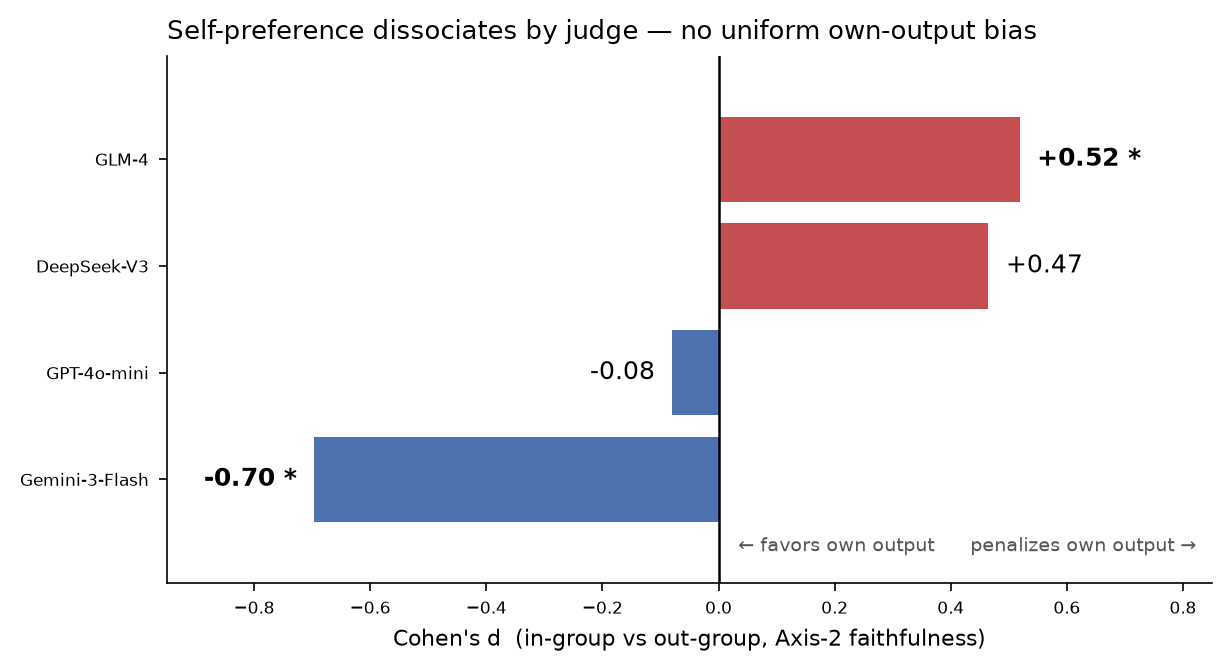
\includegraphics[width=0.95\textwidth]{Fig5_judge_self_preference_v2.png}
\caption{Left: judge leniency on the 108-item shared sample, non-blind vs.\ blind, on A2. Right: in-group vs.\ out-group A2 means under the blind condition, with Cohen's $d$ annotated. Negative $d$ indicates self-favoring; positive $d$ indicates self-penalizing.}
\label{fig:judge}
\end{figure}

\section{Discussion}

The dominant finding places most of the scoring variance upstream in the demographic prompt, with model choice contributing little. SES alone explains nearly half of the variance in PHQ-8 scores ($d=1.95$), while race and model identity together explain about 5\%. One caveat on this comparison deserves note. Being a designed, maximally-separated binary contrast (concierge/\$250k vs.\ Medicaid/\$35k), SES stands against generator identity as an incidental 4-level factor never constructed to maximize between-model spread, and the raw ``SES 48.75\% vs.\ model 2.22\%'' gap therefore partly reflects that design asymmetry rather than a pure apples-to-apples effect ranking. Even granting the caveat, the four models tested are, on this dimension, more similar than different. A practitioner choosing among them on the basis of psychological scoring fairness gains little by switching, as the bias sits upstream in how all four respond to the SES cue.

None of the explanation types tested surface this. Feature Attribution, the most common interpretability output, allocates 63.4\% of the score to ``clinical presentation'' across the three models whose FA output parsed reliably (DeepSeek, Gemini, GPT; $n=1{,}062$), and clinical presentation is the score itself. SES, the empirically dominant driver, receives 17.2\%. Being judge-independent, the FA inversion forms the robust core of this result. The complementary judge-based signal points the same way, with $31.6\%$ of explanations scoring A1$=1$ (named demographics) and A4$\geq 4$ jointly. The inversion holds across all four models, with claimed SES weights of $24.3\%$ (GPT-4o-mini), $14.9\%$ (Gemini-3-Flash), $12.3\%$ (DeepSeek-V3), and $5.1\%$ (GLM-4.7) against a true SES variance share of $\approx 49\%$, and GLM assigning $88.8\%$ to ``clinical presentation'' as the most extreme case. Naming the variable is not the same as attributing causal weight to it. The explanations consistently do the first while skipping the second, mirroring the broader finding that a model's stated rationale need not reflect the features that actually drive its output, both in chain-of-thought reasoning \cite{turpin2023, lanham2023} and in current reasoning models \cite{chen2025}, and that post-hoc explanations can be scaffolded to conceal rather than reveal a biased decision \cite{slack2020}.

Among the four XAI types, Abductive explanations rate best on Faithfulness and Fairwashing under the internal anchor, with Feature Attribution worst on both. Among generator models, GLM-4.7 produces the most-faithful and least-fairwashed explanations on average while DeepSeek-V3 produces the worst on both axes. GLM manages this with much longer explanations whose token count shows no relationship to judged faithfulness ($\rho=-0.02$, $p=.81$). For the other three models longer explanations do earn better faithfulness ratings ($\rho$ from $-0.50$ to $-0.66$), showing that GLM's added volume buys no rated gain.

A separate concern emerges from the judge analysis. The leniency spread between Gemini and GPT-4o-mini (1.20 points on A2) exceeds any cohort or model effect in the substantive results. A single-judge protocol fixes this scale somewhere between $2.16$ and $3.36$, meaning any reported A2 mean must be read against the chosen judge. Self-preference compounds the problem. Gemini favors its own outputs and DeepSeek penalizes its own, with both effects preserved (and possibly amplified) under blinding, though the leak-free recompute in Section 4.6 shows the blind result to be fragile and partly leak-driven. We deliberately do not frame this as a Western-versus-Eastern pattern: the other two judges contradict their regional camps and a regional test carries only $df=1$, making the finding a two-judge dissociation rather than evidence of an alignment-geography effect. Replication with several judges per region is required before any cross-cultural interpretation.

\section{Limitations and next steps}

Regarding limitations and honest caveats, three matter for the larger study. First, although the primary evaluation set carries a three-vote consensus (94.1\% three-vote, 5.9\% two-vote; $n=1{,}072$), every vote comes from the same judge model, so the consensus removes vote noise but not judge-family bias. Because the primary judge is also one of the four generators, self-preference cannot be ruled out of the headline numbers, and the full study should rotate to a non-generator primary judge while averaging across judge families. Additionally, the FA dimension labels are coarse (race, gender, SES, clinical, other), and finer-grained schemas (separating insurance status from income, or splitting clinical presentation into symptom counts and severity language) may shift the inversion result. Finally, the 108-item cross-judge sample remains small for the self-preference analysis with only two Western and two Eastern judges; the larger study should include at least four judges per region.

The pilot establishes the design's measurement floor. The cohort-substitution design produces an effect size large enough ($d \geq 1$ on PHQ-8 SES) to detect with modest sample sizes, the 4-type explanation rubric distinguishes between explanation types with $d \geq 0.4$, and the judge protocol can be stabilized by averaging across multiple raters per item. The headline result, that explanations name the variable but do not weight it, replicates across all four generators, both framings, and (under blinding) both Western judges. The full study will scale the cohort matrix, formalize the multi-judge consensus, re-run the blind self-preference analysis under a fully leak-free prompt, and add a human-rater calibration sample to anchor the LLM judges.

\section{Ethics statement}

All patient vignettes in this study are synthetic and contain no real patient data, so institutional review was not required. The four instruments are screening tools, and the model outputs studied here are not clinical assessments; the demographic score gaps we report describe model behavior on constructed cohorts and should not be read as epidemiological claims about real populations. The intended use of this audit is to inform evaluation practice for LLMs in mental-health-adjacent settings, with the finding that explanations fail to disclose demographic drivers arguing for caution before any clinical deployment.

\section{Data and code availability}

All raw datasets, analysis scripts (\texttt{01\_phase1\_generation.py} through \texttt{07\_figures.py}), result CSVs, and figures are in the project repository. The \texttt{full\_pilot}, \texttt{pilot\_n10}, \texttt{cross\_judge\_reliability}, and \texttt{blind\_judge} subdirectories contain the four datasets referenced in this report. Statistical procedures use \texttt{scipy.stats}; figures use \texttt{matplotlib}.

\appendix
\section{Analysis revisions and robustness}
\label{app:revisions}

The results above reflect the final analysis pipeline. Four revisions to earlier versions of the analysis are recorded here for completeness; none changes the direction of any reported effect.

\textbf{Fairwashing anchor.} A4 originally scored each explanation against external population epidemiology. Because that anchor conflates disagreement with epidemiology and concealment of the model's own reasoning, A4 was re-scored against the model's stated demographic adjustment (the internal anchor). Re-scoring lowered the fairwashing headline from $\bar{x}=3.49$ ($61.5\%\geq 4$, $52.2\%$ name-and-fairwash) to $\bar{x}=3.02$ ($40.3\%$, $31.6\%$), while the mean is essentially unchanged between a single vote and the three-vote consensus ($3.01$ vs.\ $3.02$). Under the internal anchor the SES effect on A4 strengthened ($d=+0.29\rightarrow+0.45$), the race effect fell to non-significance, and the framing effect did not survive, consistent with A4 tracking a surface SES cue rather than the injected epidemiological reference.

\textbf{Feature-attribution regeneration.} GLM-4.7's original feature-attribution run used a 600-token cap that truncated its JSON on 89\% of rows (40 of 350 parseable). All 350 cells were regenerated at a 2{,}000-token cap with reasoning suppressed, recovering 350/350. The regenerated GLM sharpens rather than changes the inversion (SES $5.1\%$, clinical $88.8\%$), and the three-model headline ($n=1{,}062$) is reported in the body to keep the FA figures on the fully clean subset.

\textbf{Judge provenance.} The original single-judge set contained 103 rows (9.6\%) whose Gemini consensus silently averaged in a DeepSeek fallback vote. The three-vote consensus set ($n=1{,}072$) supersedes both that set and its clean Gemini-only subset ($n=971$), which differ negligibly on every reported descriptive.

\textbf{Blinding leak.} The blind prompt named the generator inside the Transgender-Woman suppression note, so TW-cohort items were effectively un-blinded (Section 4.6). The leak-free recompute is reported alongside the leaky numbers; a fully leak-free re-run is the primary open item for the full study.

\begin{thebibliography}{99}

\bibitem{kroenke2009phq8} Kroenke, K., Strine, T. W., Spitzer, R. L., Williams, J. B. W., Berry, J. T., and Mokdad, A. H. (2009). The PHQ-8 as a measure of current depression in the general population. \textit{Journal of Affective Disorders}, 114(1--3):163--173.

\bibitem{spitzer2006gad7} Spitzer, R. L., Kroenke, K., Williams, J. B. W., and L\"owe, B. (2006). A brief measure for assessing generalized anxiety disorder: the GAD-7. \textit{Archives of Internal Medicine}, 166(10):1092--1097.

\bibitem{bush1998auditc} Bush, K., Kivlahan, D. R., McDonell, M. B., Fihn, S. D., and Bradley, K. A. (1998). The AUDIT alcohol consumption questions (AUDIT-C): an effective brief screening test for problem drinking. \textit{Archives of Internal Medicine}, 158(16):1789--1795.

\bibitem{blevins2015pcl5} Blevins, C. A., Weathers, F. W., Davis, M. T., Witte, T. K., and Domino, J. L. (2015). The Posttraumatic Stress Disorder Checklist for DSM-5 (PCL-5): development and initial psychometric evaluation. \textit{Journal of Traumatic Stress}, 28(6):489--498.

\bibitem{aivodji2019fairwashing} A\"ivodji, U., Arai, H., Fortineau, O., Gambs, S., Hara, S., and Tapp, A. (2019). Fairwashing: the risk of rationalization. In \textit{Proceedings of the 36th International Conference on Machine Learning (ICML)}, PMLR 97:161--170.

\bibitem{jacovi2020faithfulness} Jacovi, A. and Goldberg, Y. (2020). Towards faithfully interpretable NLP systems: how should we define and evaluate faithfulness? In \textit{Proceedings of the 58th Annual Meeting of the Association for Computational Linguistics}, pages 4198--4205.

\bibitem{miller2019explanation} Miller, T. (2019). Explanation in artificial intelligence: insights from the social sciences. \textit{Artificial Intelligence}, 267:1--38.

\bibitem{wachter2018counterfactual} Wachter, S., Mittelstadt, B., and Russell, C. (2018). Counterfactual explanations without opening the black box: automated decisions and the GDPR. \textit{Harvard Journal of Law \& Technology}, 31(2):841--887.

\bibitem{zheng2023judging} Zheng, L., Chiang, W.-L., Sheng, Y., Zhuang, S., Wu, Z., Zhuang, Y., Lin, Z., Li, Z., Li, D., Xing, E. P., Zhang, H., Gonzalez, J. E., and Stoica, I. (2023). Judging LLM-as-a-judge with MT-Bench and Chatbot Arena. In \textit{Advances in Neural Information Processing Systems 36}, Datasets and Benchmarks Track.

\bibitem{zack2024gpt4bias} Zack, T., Lehman, E., Suzgun, M., Rodriguez, J. A., Celi, L. A., Gichoya, J., Jurafsky, D., Szolovits, P., Bates, D. W., Abdulnour, R.-E. E., Butte, A. J., and Alsentzer, E. (2024). Assessing the potential of GPT-4 to perpetuate racial and gender biases in health care: a model evaluation study. \textit{The Lancet Digital Health}, 6(1):e12--e22.

\bibitem{bouguettaya2025racialbias} Bouguettaya, A., Stuart, E. M., and Aboujaoude, E. (2025). Racial bias in AI-mediated psychiatric diagnosis and treatment: a qualitative comparison of four large language models. \textit{npj Digital Medicine}, 8:332.

\bibitem{turpin2023} Turpin, M., Michael, J., Perez, E., and Bowman, S. R. (2023). Language models don't always say what they think: unfaithful explanations in chain-of-thought prompting. In \textit{Advances in Neural Information Processing Systems 36}.

\bibitem{lanham2023} Lanham, T., Chen, A., Radhakrishnan, A., Steiner, B., Denison, C., Hernandez, D., Li, D., Durmus, E., Hubinger, E., Kernion, J., Lukošiūtė, K., Nguyen, K., Cheng, N., Joseph, N., Schiefer, N., Rausch, O., Larson, R., McCandlish, S., Kundu, S., Kadavath, S., Yang, S., Henighan, T., Maxwell, T., Telleen-Lawton, T., Hume, T., Hatfield-Dodds, Z., Kaplan, J., Brauner, J., Bowman, S. R., and Perez, E. (2023). Measuring faithfulness in chain-of-thought reasoning. \textit{arXiv:2307.13702}.

\bibitem{chen2025} Chen, Y., Benton, J., Radhakrishnan, A., Uesato, J., Denison, C., Schulman, J., Somani, A., Hase, P., Wagner, M., Roger, F., Mikulik, V., Bowman, S. R., Leike, J., Kaplan, J., and Perez, E. (2025). Reasoning models don't always say what they think. \textit{arXiv:2505.05410}.

\bibitem{atanasova2023} Atanasova, P., Camburu, O.-M., Lioma, C., Lukasiewicz, T., Simonsen, J. G., and Augenstein, I. (2023). Faithfulness tests for natural language explanations. In \textit{Proceedings of the 61st Annual Meeting of the Association for Computational Linguistics (Volume 2: Short Papers)}, pages 283--294.

\bibitem{slack2020} Slack, D., Hilgard, S., Jia, E., Singh, S., and Lakkaraju, H. (2020). Fooling LIME and SHAP: adversarial attacks on post hoc explanation methods. In \textit{Proceedings of the AAAI/ACM Conference on AI, Ethics, and Society (AIES)}, pages 180--186.

\bibitem{ribeiro2016lime} Ribeiro, M. T., Singh, S., and Guestrin, C. (2016). ``Why should I trust you?'': explaining the predictions of any classifier. In \textit{Proceedings of the 22nd ACM SIGKDD International Conference on Knowledge Discovery and Data Mining}, pages 1135--1144.

\bibitem{lundberg2017shap} Lundberg, S. M. and Lee, S.-I. (2017). A unified approach to interpreting model predictions. In \textit{Advances in Neural Information Processing Systems 30}, pages 4765--4774.

\bibitem{rudin2019} Rudin, C. (2019). Stop explaining black box machine learning models for high stakes decisions and use interpretable models instead. \textit{Nature Machine Intelligence}, 1:206--215.

\bibitem{panickssery2024} Panickssery, A., Bowman, S. R., and Feng, S. (2024). LLM evaluators recognize and favor their own generations. In \textit{Advances in Neural Information Processing Systems 37}.

\bibitem{wang2024} Wang, P., Li, L., Chen, L., Cai, Z., Zhu, D., Lin, B., Cao, Y., Kong, L., Liu, Q., Liu, T., and Sui, Z. (2024). Large language models are not fair evaluators. In \textit{Proceedings of the 62nd Annual Meeting of the Association for Computational Linguistics (Volume 1: Long Papers)}, pages 9440--9450.

\bibitem{saito2023} Saito, K., Wachi, A., Wataoka, K., and Akimoto, Y. (2023). Verbosity bias in preference labeling by large language models. \textit{arXiv:2310.10076}.

\bibitem{gu2024} Gu, J., Jiang, X., Shi, Z., Tan, H., Zhai, X., Xu, C., Li, W., Shen, Y., Ma, S., Liu, H., Wang, Y., and Guo, J. (2024). A survey on LLM-as-a-judge. \textit{arXiv:2411.15594}.

\bibitem{omiye2023} Omiye, J. A., Lester, J. C., Spichak, S., Rotemberg, V., and Daneshjou, R. (2023). Large language models propagate race-based medicine. \textit{npj Digital Medicine}, 6:195.

\bibitem{gallegos2024} Gallegos, I. O., Rossi, R. A., Barrow, J., Tanjim, M. M., Kim, S., Dernoncourt, F., Yu, T., Zhang, R., and Ahmed, N. K. (2024). Bias and fairness in large language models: a survey. \textit{Computational Linguistics}, 50(3):1097--1179.

\bibitem{blodgett2020} Blodgett, S. L., Barocas, S., Daum\'e III, H., and Wallach, H. (2020). Language (technology) is power: a critical survey of ``bias'' in NLP. In \textit{Proceedings of the 58th Annual Meeting of the Association for Computational Linguistics}, pages 5454--5476.

\bibitem{singh2024} Singh, S., Keshari, S., Jain, V., and Chadha, A. (2024). Born with a silver spoon? Investigating socioeconomic bias in large language models. \textit{arXiv:2403.14633}.

\bibitem{an2025} An, J., Huang, D., Lin, C., and Tai, M. (2025). Measuring gender and racial biases in large language models: intersectional evidence from automated resume evaluation. \textit{PNAS Nexus}, 4(3):pgaf089.

\end{thebibliography}

\end{document}
